\chapter{Design}
% introduction about the network stack?

\section{Overview}
The networking stack introduced in this thesis is implemented in the C\# 
programming language with SME. The aim of its design is to capacitate performance,
flexibility, and ease of use. In this chapter, the design principles are 
described, the architecture of the solution is outlined, and the components are
outlined.


\subsection{Design principles}
As briefly mentioned in the introduction, the proposed network stack is to 
provide an alternative to the existing proprietary network offloading engines.
While the main goal of this thesis is to research and study the suitability of 
SME for implementing a TCP/IP stack on an FPGA, there are many other aspects of the 
system to be studied.\\
The extensibility of the network stack are to be tested by studying the effects 
of introducing new protocols to the stack. While the network stack should be 
able to be refined with new and custom protocols, it is to be studied which 
implications it has for the system. Mainly, it is to be seen how the addition 
of new protocols affect the performance, scalability, and viability of the 
system.\\
In the same vein, the design should be as FPGA-agnostic as possible. While this is 
mainly guaranteed by the SME framework used to develop the system, the underlying
systems, operations, and features should be easily portable across FPGA manufacturers.\\
Lastly, the design of the networking stack should be interoperable with other 
systems on the FPGA, or even FPGAs. It is to be seen how easy it us to modify
and extend the versatility of the system without any major modifications or 
even extensible knowledge of the system. As an example, the networking stack 
can be expanded with a firewall, developed alongside this project. 

\subsection{Initial requirements}
Following our design principles, initial requirements and goals for the 
networking stack are set so that these can be tested and improved upon. 
\begin{itemize}
\item \textbf{Essential protocols only}\\
Considering that the SME project is still fairly early in its development, and considering 
the sheer number of protocols in the internet protocol suite, the networking 
stack in this thesis is to support only the absolutely essential protocols 
required to provide the users with a meaningful interface to the internet.
These protocols should be picked such that the system can provide the end-user
with a network data-stream, which can transport information to and from a remote
computer.\\
The initial protocols chosen may be implemented and supported partially, but 
they must not deviate from the standard specifications. 

\item \textbf{Support an interface for the end-user}\\
The system must be controlled by an end-user on the FPGA. Such an interface is 
very unique in its own way, compared to standard software interfaces, like the 
ones defined in the POSIX collection of specifications. By supporting such an
external interface gains insight in the way such a networking stack will be used,
and which measures must be taken in order to provide the best possible integration
and performance considerations.

\item \textbf{Independent of underlying physical hardware}\\
By using SME, the underlying hardware description language code can be abstracted
away from the actual implementation. This will later provide developers to easily
modify and tweak the networking stack without having to consider the target 
hardware.\\
Likewise, the networking stack may not rely on using a certain physical layer hardware,
and must be designed to be independent of the underlying hardware used for the 
physical connections. This will ensure that the target hardware can easily 
swap between physical connectors, such as going from ethernet cables to wireless,
or even another FPGA.
\end{itemize}

\section{Initial design}

% Spans 2 columns
\begin{figure*}
    \centering
    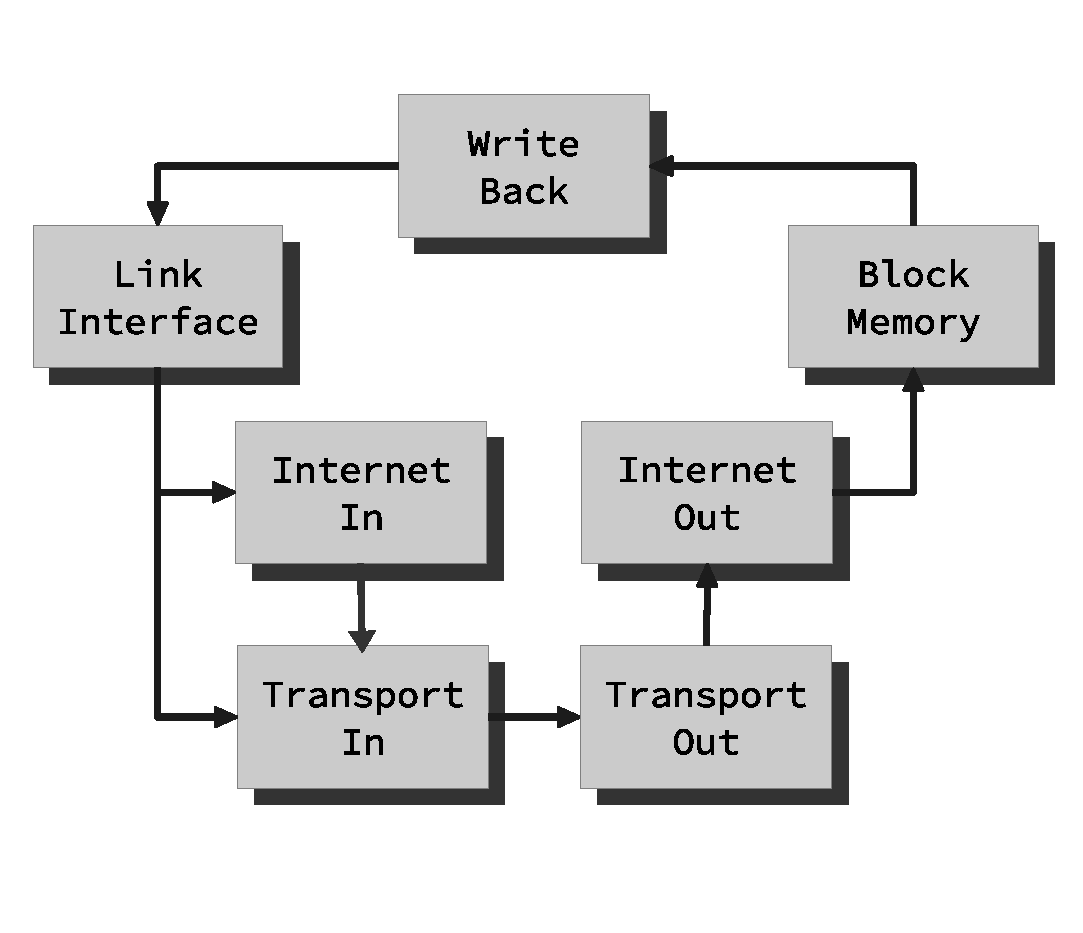
\includegraphics[scale=0.45]{design/design_0.eps}
    \caption{The initial design}
    \label{fig:initial_design}
\end{figure*}

The initial architecture had a very simplistic approach to its design in order 
to aid with early identification of potential issues and problems. 
The basic idea of the initial design is to minimize the number of memory 
operations carried out. Under the assumption that the Ethernet interface used in the network 
stack will likely have limited memory, everything needs to be copied directly to
the stack. Figure \ref{fig:initial_design} shows the initial design, where the 
leftmost module Ethernet connects to the memory for direct access, and each 
parsing layers listens to this connection and performs accordingly. Each parsing 
layer also connects to the subsequent layer in order to flag when the subsequent
layer should start listening on the data-bus (that is, where the current packet
header stops and the next header begins).\\
An advantage that this design provided was the cetralized memory, which is much 
easier to up-scale in terms of capacity and bandwidth. This global memory would 
also be able to modify packets in-place, removing duplicate data, minimizing the 
need to copy data around, and making it easier to keep track of the memory 
fragmentation.

\subsection{The issues}
As anticipated, this initial design brought fourth the main issue fairly quickly 
in the implementation phase, where most of these stem from the differences in 
programming hardware as opposed to the software network stack, from which the 
inspiration was drawn.

\subsubsection{Internal parsing buffer or memory is largely unavoidable}
Although listening to the global data-bus and processing on the bytes currently 
therein  seems like an efficient way of minimizing the data-transfer required 
across processes, it has shown to yield some unavoidable challenges.\\
Parsing fields in a packet-header is much more cross-dependent than initially 
anticipated; each field might have numerious implications on the way preceeding 
and subsequent fields are read and interpreted. As an example, in the Internet
Control Message Protocol (ICMP), a redirect message type has an IPv4 address field in 
the header, whereas in the timestamp message type, this field is interpreted as 
both an identifier and a sequence number.
This sort of inter-dependency is hard to parse without the ability of caching 
or buffering the header locally in the parsing process. 

\subsubsection{Overutilized memory module}
While the ethernet is the main writer to the memory module, the parsing layers 
need to access and write to the module as well. At the very least, the memory 
module would have 6 connections in the network, not counting any additional 
components, such as user interface, firewall, etc. 
Although numerous memory implementations exist on the FPGA landscape, Block RAM 
(BRAM) seems to be the most suitable in this situation for its speed and latency.
Unfortunately, many widely used block RAMs only have 2 simultaneous connections 
(or "ports") at the same time. Additionally, the block rams are frequently 
limited to only operate a few bytes of data at a time.\\
Although some block RAMs, such as the ones found in Xilinx FPGAs can be cascaded\cite{xilinx_fpga_memory_resources}
to lessen the impact of these limitations, this hardly provides a good basis for 
a scalable design.

\subsubsection{Data fragmentation and memory management}
Another problem a unified address space in the global memory is how costly 
basic memory operations, such as moving or copying, become. The initial 
assumption that packets stored in memory could be reused by modifying them 
in-place and send them turned out to be misguided, since the layout, size, and 
the number of the outgoing packets very rarely resemble the in-going packets.\\
Furthermore, the general purposeness of the memory makes it very hard to 
structure. Without very complex memory management, the memory can get very 
fragmented and slow.


\section{Revised design}
The initial architecture focused heavily on the input from the link interface, 
minimizing hardware memory requirements, and to minimize the latency from the 
source data-stream to its respective layer handler. Unfortunately, the opposite 
revealed to be true, as the overly-utilized memory unveiled plentiful issues to 
the performance.\\

\begin{figure}[h]
    \centering
    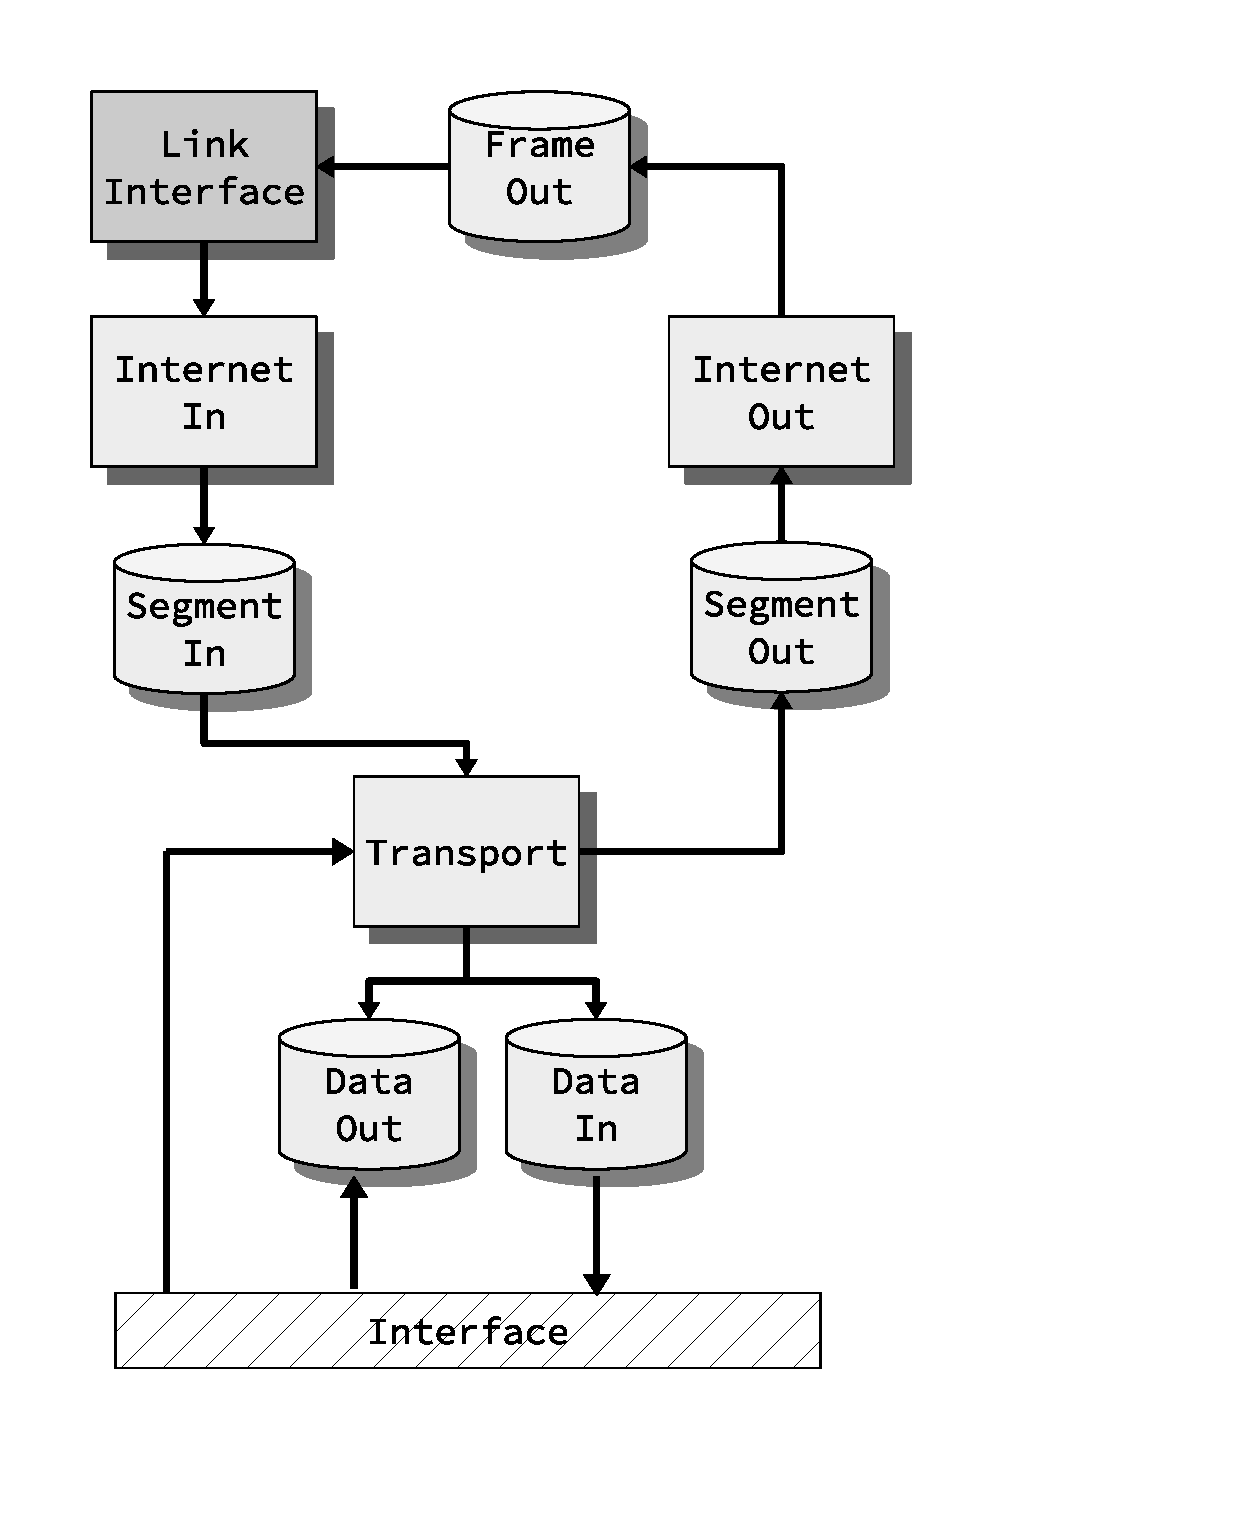
\includegraphics[scale=0.45]{design/design_1.eps}
    \caption{Second iteration of the design}
    \label{fig:second_design}
\end{figure}

To avoid the problem with global memory, the data needs to "flow" through the 
components that need the data at that time. Therefore, as opposed to the initial 
design, where the link interface writes to memory directly, in the revised design, 
this connection is completely removed. The idea is to let all the data pass 
pass through each state, letting each stage parse the required information, and 
passing the rest to the next components.\\
As seen on figure \ref{fig:second_design}, the link interface, which
provides the raw byte-stream from the network, is connected to all of the input
parsing layers. The layers are connected in the order in which a network frame 
is parsed; link- to internet- to transport-layer. This approach aims to utilize
the fact that the layers can act immediatelly upon the packets received directly
from the source, avoid having to buffer the whole packet in each stage, as well 
as easing the logic required to buffer the data across the layers.\\
This design starts by the Link Interface sending one byte at a time through its bus. 
The \texttt{Link In} will parse the first header, and signal the next layer upon completion.
\texttt{Internet In} will then start to listen on the \texttt{Link Interface} bus
and, using the information from \texttt{Link In}, parse the internet header 
accordingly. The same procedure would be applied to the connection between 
\texttt{Internet In} and \texttt{Transport In}.\\
When data is to be sent to the internet, the network frame would be built bottom
up from the transport layer through internet to the link layer.

\subsection{The issues}
The issues quickly surfaced during the implementation of this revised design. Although 
the interconnect from the \texttt{Link Interface} to all the subsequent layers
in parallel promised negligible latency, it came with a great cost to the solution.

\subsubsection{Process under-utilization} \label{item:process_utilization}
Since each "in" process has to wait for the previous layer to signal when to 
start listening on the data-bus, the layers would in average only be active a third
of the time. Since each layer has very little information about the states of 
the other layers, it would become a challenge to get any other work done during
these phases.\\
For example, it would be an immense challenge to coordinate an ICMP reply on a 
faulty packet in the \texttt{Internet In}.

\subsubsection{Redundant Link layer}
While the Link layer is an essential part of the Internet Protocol Suite, it did 
not fit well with the functionality of the rest of the stack. 
Most network interfaces are equipped with buffers, on which integrated circuits
perform operations such as error check using cyclic redundancy check, de-noising,
timeslot management, etc. 
Likewise, the Pmod NIC100 Ethernet interface has built-in controller with 
internal memory suited for buffering the incoming packets\cite{microchip_enc424j600}.
This memory, apart from the cyclic redundancy check, can be used as the initial
step for parsing the packet, and only send the datagram to the stack.


\subsubsection{IPv4 fragmentation and out of order TCP packets}
The chaotic nature of internet routing might cause packets to come out of order,
or even get fragmented along the way. Since each layer parses the packet immediatelly
as it is written to the bus, it became a challenge for the layers to figure out 
what to do. On IPv4 fragmentation, if the second half of a dataframe arrived 
first, the Transport header would not be available to the Transport layer. 
Although IPv4 fragmentation is an increasingly rare phenomenon, the network 
design is not able to handle the situation well.  


\subsubsection{TCP connection state sharing}
With a clear separation between the "in" layers and the "out" layers, the 
Transport block had to be split as well. Unfortunately, unlike the other stateless
layers, the transportl layer actually needs to keep track of the connections and 
their states. On every segment received, the appropriate connection needs to be 
updated accordingly.\\
In the TCP protocol, the connection state changes on both receiving and sending.
In this case, the \texttt{Transport In} and \texttt{Transport Out} have to 
agree on a shared state. As these states can be quite large, and the should 
support multiple connections at once, one large bus containing all the information
is not feasible. To solve this, a negotiation protocol may be introduced, however,
as pointed out in item \ref{item:process_utilization}, the processes are very
limited in their execution time. A negotiation would be very hard to achieve in 
such circumstances.


\subsubsection{Problematic order of building and sending outgoing packets}
Outgoing packets are built in the reverse order of which they are parsed -- the 
inner layers are built first, and then the packet grows outwards by adding new 
layers on top of the existing one.\\
That in itself is not a problem, as the packet can be easily passed through the 
network backwards from the last byte first.
However, this would require that the network knows the length of the data-section
of the packet beforehand, as it needs to know which user data-byte to start from.
Unfortunately, knowing where to start prior to sending is not a trivial, nor is 
it very efficient or practical. 
For improved performance and flexibility, it is better to just let the 
stack send as much data out as possible with as little overhead as possible.\\
Figure \ref{fig:sending_packet_order} shows the possible ways of creating and 
passing a packet along the network stack. 
\begin{figure}
    \centering
    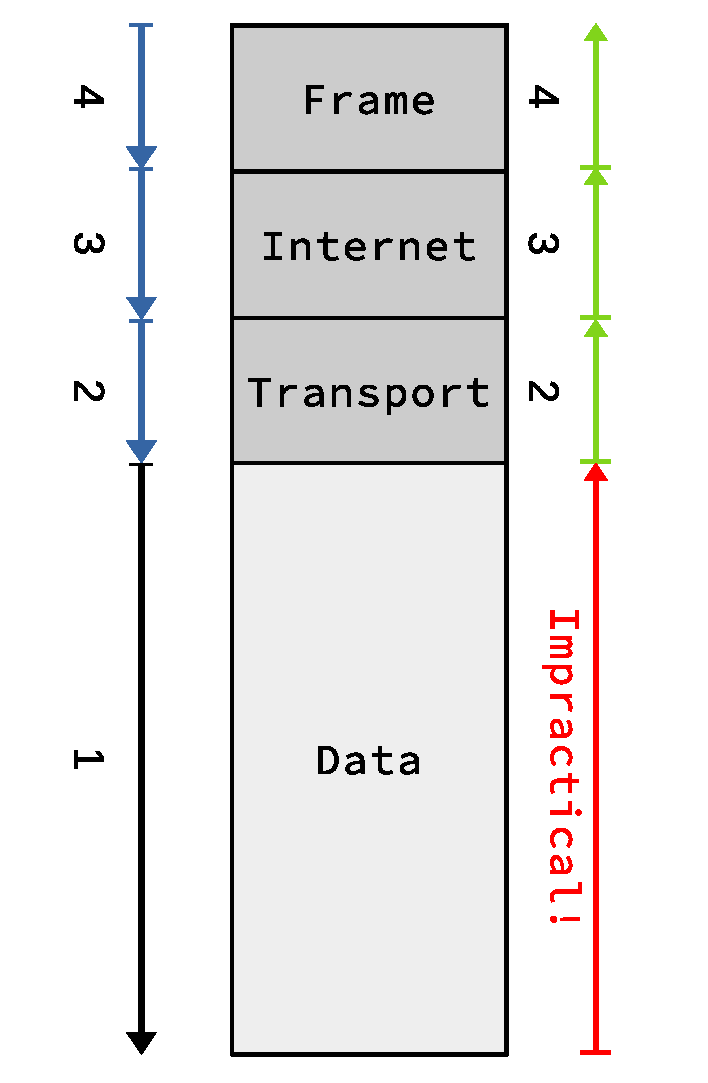
\includegraphics[scale=0.45]{design/sending_packet_order.eps}
    \caption{Possible orders of ways of building an outgoingg packet}
    \label{fig:sending_packet_order}
\end{figure}

While the right side of figure \ref{fig:sending_packet_order} is more intuitive,
it is impractical for the reasons described above. The left side is better 
performance-wise, but slighty more odd in the way bytes are added without any 
sequential order.


% \subsubsection{Control and logic flow}
% Although the layers take turns to parse the incoming byte-stream, the design 
% handles the whole packets at once. This leaves 

\section{Pipelined design}
While it would be possible to work around these identified issues with the 
revised design in the code, the 
added complexity would have additional ramifications on the project as a whole.
Upon further analysis of analysis, it is clear that the source of the issues is 
the parallel arrangement of the process blocks.



\begin{figure}
    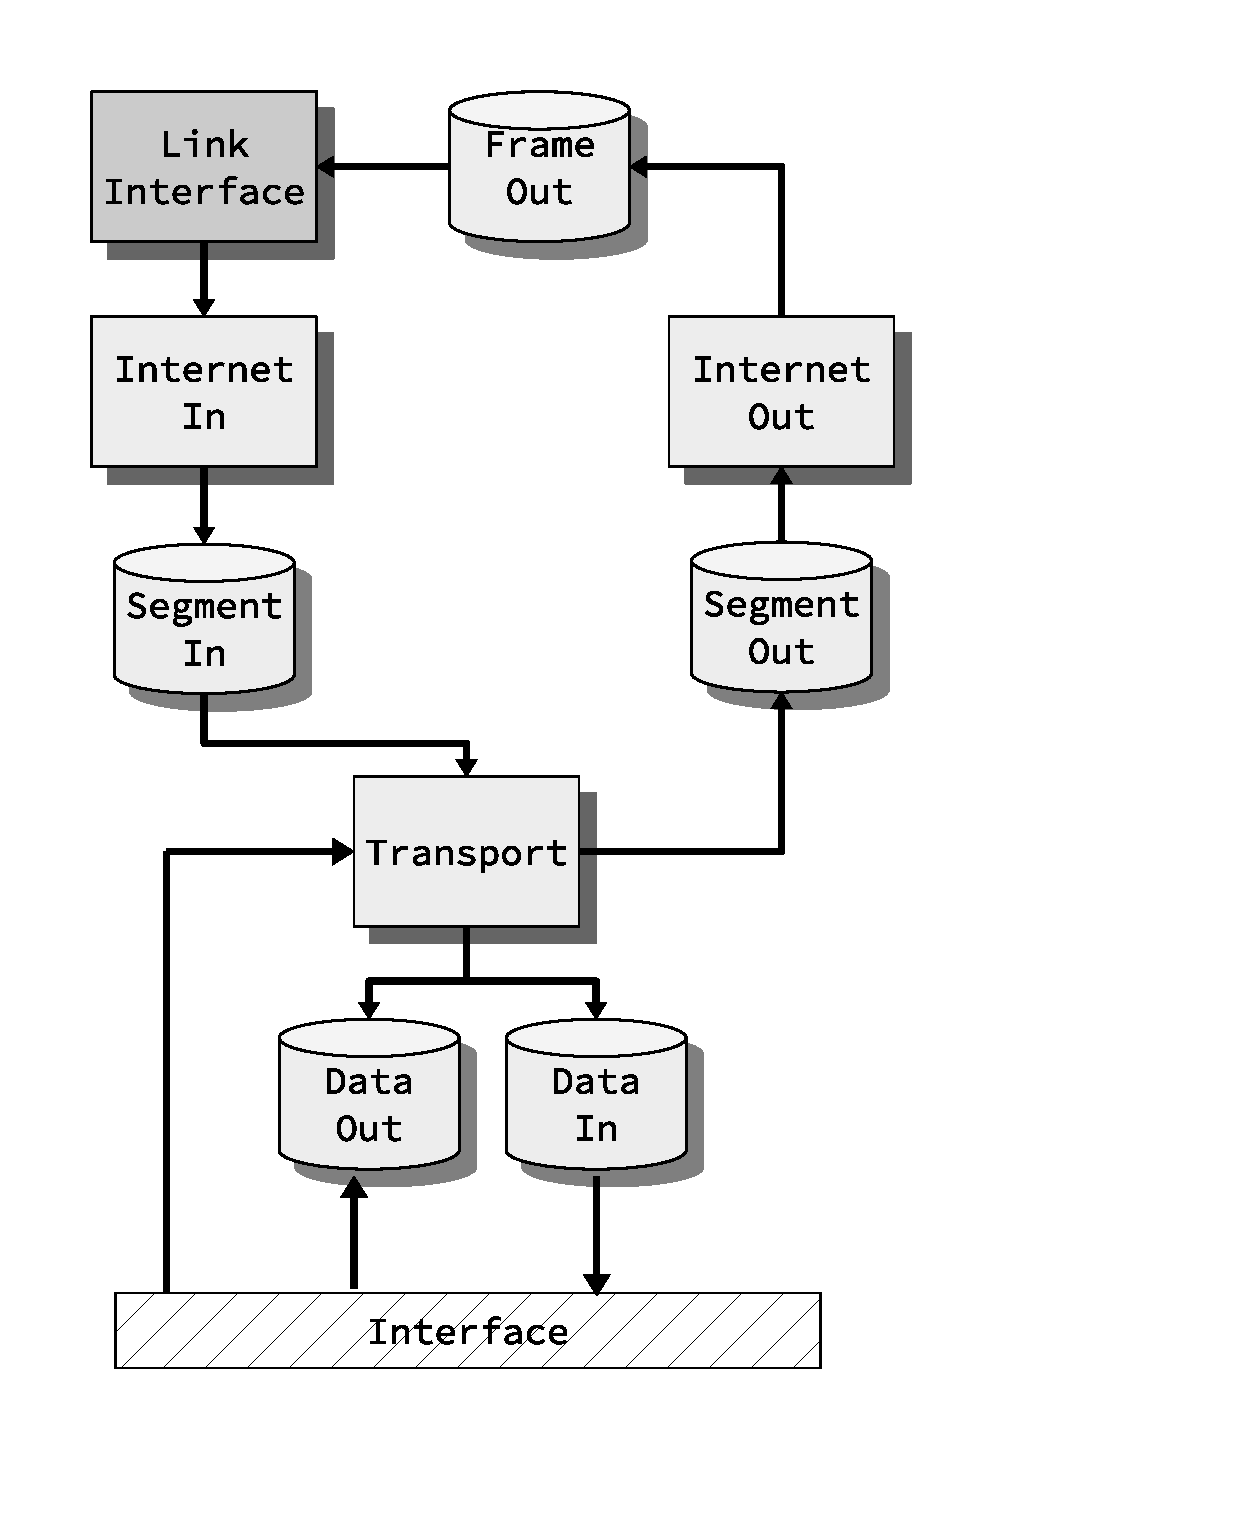
\includegraphics[scale=0.45]{design/design_2.eps}
    \caption{The final design}
    \label{fig:final_design}
\end{figure}

The next iteration of the design utilizes a fairly standard approach to 
pipelining, albeit with an unusual transfer of data between the stages.\\
The idea with the pipeline is to enable the processes to receive, compute, and 
forward data at their own pace, without any major limitation from the other 
parts of the system.


\subsection{Internet layer processes} \label{sec:layer_processes}
The processes performing computation and processing on the actual internet 
packets, called "layer processes" for brevity, are by large kept intact from the 
previous design. The fairly simple, but highly sequential nature of packet 
header parsing turned out to be very complicated to optimise with the additional
computing power of the hardware, without introducing too much complication.\\
Missing from the updated figure \ref{fig:final_design} are the \texttt{Link In}
and \texttt{Link Out} processes, which, for now, are made by the ethernet 
interface, which can easily parse and strip the first frame headers.

\subsection{Busses}
The busses in the revised pipelined design are devised such that communication 
is only limited to the immediate neighbours in the logical network. This design
is put in place so that the synchronization and the order of execution is much 
easier to keep track of, so that fewer race-conditions occur, and so that blocks 
in the network are easier to replace, remove, or modify, without having a large
cascade effect on the whole network, as opposed to only the neighbours.\\
Whereas in the previous design where the busses would simply write new data on
every new clock-cycles regardless of the reading processes, now there must be 
some logic to actually ensure that the reading process is ready to receive new 
data. While the Data Buffers, as introduced in the next section \ref{sec:data_buffers},
solve the issue of blocks reading and writing data at their own pace, the busses
must support an interface for sharing the state of both processes. Thus, while 
the busses are depicted as directional with arrows in figure \ref{fig:final_design},
there is naturally a need for a control signal in the opposite direction to 
control the data-flow. This communication protocol will be discussed further in 
the implementation section \ref{sec:interface_signal_protocol}.


\subsection{Data buffers} \label{sec:data_buffers}
Illustrated as cylinders on figure \ref{fig:final_design}, First-In, First-Out (FIFO)
buffers are introduced between each parsing process in order to control the data-flow 
between the layers. Apart from maintaining a fairly large memory bank through 
the block-RAM, these buffers also contain logic to store the incoming data
intelligently in order to offload the following processes. For example, the
\texttt{Segment In} buffer ensures that fragmented IPv4 packets are defragmented
before leaving the buffer.
However, introducing a new "type" of a process --- the buffers --- poses a new 
challenge. While the buffers can be read from at any time, the layer-parsing
processes do not have this luxury, as they do not have any significant internal
buffer. Here again it becomes obvious that a handshake protocol needs to be used 
in the bus-communication between the buffers and the processes.


\subsection{Interface}
Lastly, the Interface is designed so that the end users and system can utilize
and use the network stack.\\
The networking stack is controlled with 3 connections (consisting of bus-pairs): 
the control-, the read-, and the write-connection. While the last two connections 
are incredible simple and only transfer data from the \texttt{Data} buffers, 
the last connection controls the whole network-stack.

\subsubsection{Read/Write interface}
In conventional programming languages, the user would usually supply the a 
function call with an array or a list on which the function can operate.
However, in hardware, this is generally not the case, as arrays are costly to 
transmit at once.\\
Therefore, the two read and write interfaces would simply stream one byte at a 
time, and it is up to the user to be prepared to read or write the data.


\subsubsection{Interface Control Bus}
The Interface Control Bus controls all the "business" logic of the network -- 
maintaining the active connections, starting and closing connections, and various
other protocol-specific control on each connection.\\ 
Currently, all this can be handled by the \texttt{Transport} block which has all 
the necessary information to handle the interface requests.\\
The design of the Interface is based on the widely adopted Berkeley Sockets library,
which saw the first implementation in 4.2BSD, and has been defacto a standard 
component in the POSIX specification\cite{tcpip_illustrated_vol2}. There are 
multiple reasons for this decision:
\begin{itemize}
\item The Interface will feel more familiar to users accustomed to the Berkely 
Sockets API commonly found in mainstream systems such as Linux, OSX, and BSD 
variants.

\item The inner workings of the stack will be more transparent, and the API 
exposes fairly fine-tuned control over the whole network stack.

\item Even with the relatively few functions exposed, the API
has thrived in the most used systems as of now. It would be an understatement to 
say that the Berkeley Sockets API have stood the test of time, and therefore, it
is a good basis for the interface used in the network stack.

\end{itemize}

The first version of the stack should support the following functions:
\begin{description}
\item[\texttt{listen(protocol, port)}]\hfill\\
    Finds and initializes a free socket with the given protocol and port. This 
    socket is immediatelly put into listen mode.
    Returns error if protocol is not supported, if port taken, or if no free sockets 
    are available.
\item[\texttt{connect(protocol, ip, r\_port , l\_port])}]\hfill\\
    Connects to a remote endpoint on \texttt{ip:remote\_port} using \texttt{protocol}.
    This call is used mainly by connection-based protocols that need to 
    establish a connection before exchangning data, although it can also be used 
    by datagram-based protocols as a way of setting the default destination to
    send subsequent data to.
    Returns error if protocol is not supported, if no free sockets are available,
    or if the optional local port is taken.

\item[\texttt{accept(socket)}]\hfill\\
    Accepts the pending connection and sets up the underlying socket state 
    accordingly. Note that unlike the POSIX implementation of \texttt{accept},
    which returns a new socket with the connection, this implementation changes 
    the state of the current, listening, socket.
    Returns error if no pending connection to accept, or if invalid socket 
    supplied.

\item[\texttt{send(socket, byte, [ip], [port])}]\hfill\\
    Queues a byte for sending through the socket. An optional IP address and 
    port can be specified in certain connectionless protocols. 
    Guaranteed to succeed, given that the transport-bus can be written to. More 
    on this discussed later.  
\item[\texttt{recv(socket)}]\hfill\\
    Reads (or "receives") a single byte from the socket. The appropriate error
    code is set if no byte available on that particular socket.

\item[\texttt{close(socket)}]\hfill\\
    Closes the connection on \texttt{socket} and frees the socket for further 
    usage. Calling on an already closed on non-existent socket has no effect.
    Guaranteed to succeed.

\end{description}

While the arguably most essential functions have been defined, there are some 
functions from the Berkeley Sockets API that have been omitted for purely 
technical and practical reasons.\\
The function \texttt{socket()} is mainly used to allocate and create new sockets 
in an environment, but given that the hardware network stack has static allocation
of the sockets, it is not needed.\\
Additionaly, the \texttt{bind()} function is also missing for the sole reason 
that in the current implementation of the network stack does not have any valid 
reason not to bind a socket immediatelly.


% \cofeAm{0.7}{0.75}{2}{80}{0}

